\chapter{Solution approach} \label{chap:solution-apporach}

% ~~~~~~~~~~~~~~~~~~~~~~~~~~~~~~~~~~~~~~~~~~~~~~~~~~~~~~~~~~~~~~~~~~~~~~~~~~~~~~~~~~~~~~~~~~~~~~~~~~~~~~~~~~~
\section{Baseline solution}

\begin{itemize}
    \item Adapt existing simple indicators to detect bottlenecks.
        All the indicators consider the relationship between the processing times of jobs on the machines
        and the total (or idle) time.
        
        This idea is still applicable on the \ac{rcpsp}. However, given that the machine load can be variable
        through time, a binary \enquote{processing-idle} differentiation between machine states does not
        provide a sufficient machine-load indication.

        \cref{fig:MachineLoad} illustrates the difference between the variability of the load
        of a Job Shop machine (subfigure \ref{fig:MachineLoad:JS}) and that of a \ac{rcpsp}
        (subfigure \ref{fig:MachineLoad:RCPSP}).

    \begin{figure}[t]
      \centering

      \subfloat[Job Shop]{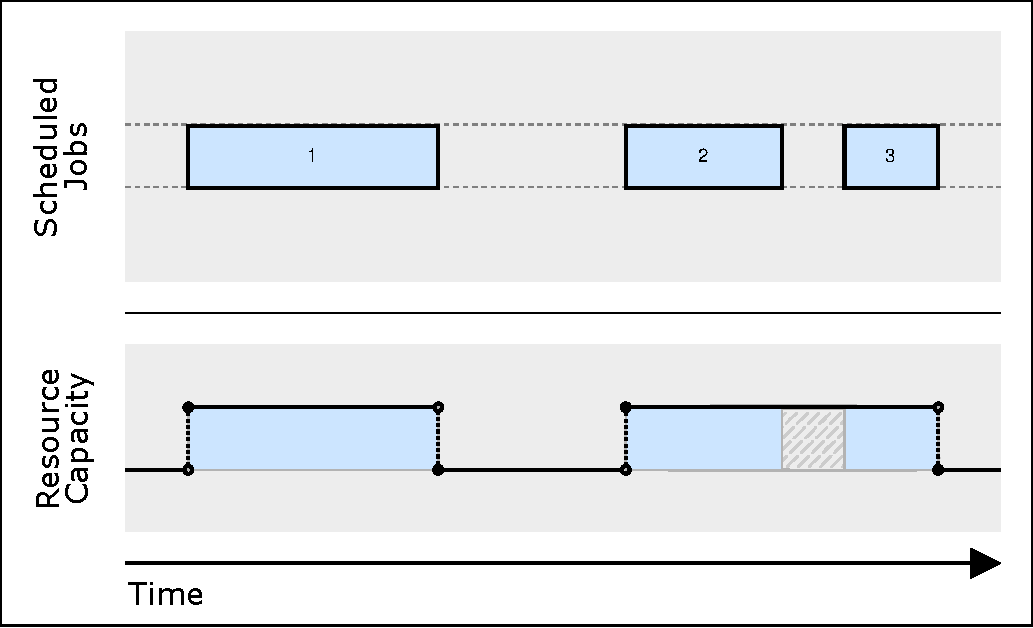
\includegraphics[width=0.7\textwidth]{img/Capacities-JobShop.pdf}\label{fig:MachineLoad:JS}}
      \\
      \subfloat[RCPSP]{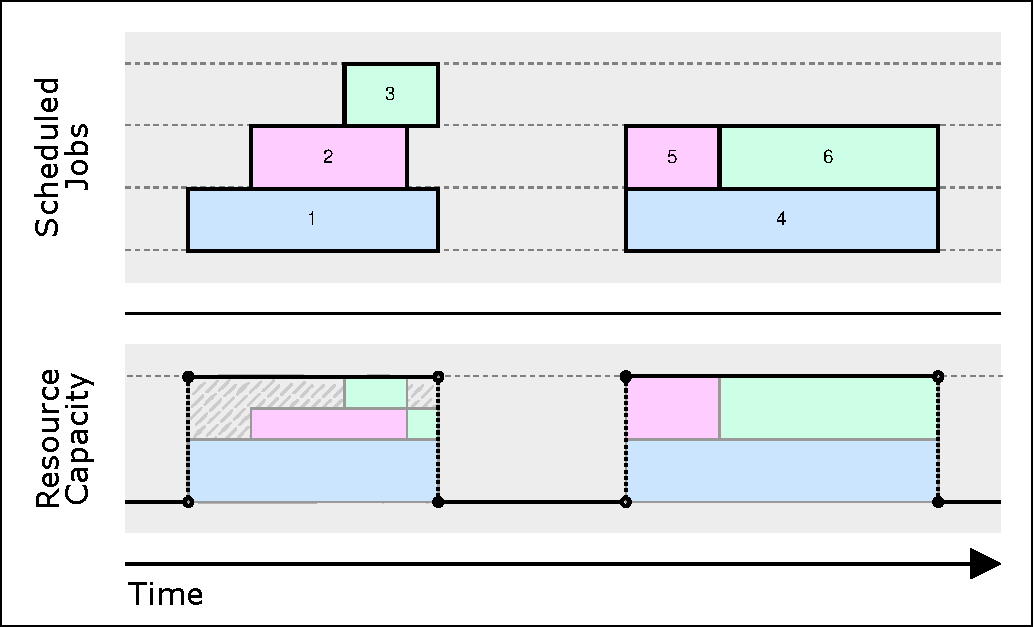
\includegraphics[width=0.7\textwidth]{img/Capacities-RCPSP.pdf}\label{fig:MachineLoad:RCPSP}}

      \caption{Caption.}
      \label{fig:MachineLoad}
    \end{figure}

    We adapt \ac{mw}, \ac{mur}, and \ac{auad} indicators (defined in \todo{ref Related works}) respectively as follows:
    \begin{itemize}
        \item \ac{mrw}
        $$
        \indMRW{k} = \sum_{\substack{j \;:\; \text{$j$ consumes $k$}}} p_j \; r_{jk}
        $$

        \item \ac{mrur}
        $$
        \indMRUR{k} = \frac{\indMRW{k}}{R_k \; (\max_{j \;:\; \text{$j$ consumes $k$}} C_j - \min_{j \;:\; \text{$j$ consumes $k$}} S_j)}
        $$

        \item \ac{auac} \todo{this might be a bit harder}
        $$
        \indAUAC{k} = \begin{cases}
            \frac{\sum_{a \in A_k} \text{consumption in $a$}}{\abs{A_k}} & \dots \text{consumption} \\
            \frac{\sum_{a \in A_k} (\text{consumption in $a$}) / (\text{capacity} \cdot \abs{a}))}{\abs{A_k}} & \dots \text{consumption to capacity ratio} \\
            \frac{\sum_{a \in A_k} (\text{consumption in $a$}) / (\text{capacity}))}{\abs{A_k}} & \dots \text{consumption to capacity ratio times the period length}
            \end{cases}
        $$
    \end{itemize}

    \item Metric-based evaluation algorithm:
    \begin{steps}
        \item We select an evaluation metric and a one-dimensional convolution mask.
        \item The solution is evaluated using the selected metric. \label{enum:metric-evaluation}
        \item A resource with an extremal metric value is selected as the bottleneck resource.
        \item Granularized period consumption is computed for the resource.
        \item The granularized consumption is convolved with the selected convolution mask to compute
            an improvement potential for each period.
        \item A predefined maximum number of periods is selected for improvement,
            selecting with respect to their corresponding improvement potential.
        \item The capacity of the bottleneck resource is increased by a predefined value
            during each of the selected improvement periods.
        \item An alternative solution of the modified instance is found and the capacity changes
            are reduced to only include the utilized capacity.
        \item Repeat from \cref{enum:metric-evaluation} for a predefined number of iterations.
    \end{steps}
\end{itemize}

% ~~~~~~~~~~~~~~~~~~~~~~~~~~~~~~~~~~~~~~~~~~~~~~~~~~~~~~~~~~~~~~~~~~~~~~~~~~~~~~~~~~~~~~~~~~~~~~~~~~~~~~~~~~~
\section{Extended solution}

We propose a procedure which detects bottlenecks in the schedule and relaxes those bottlenecks to obtain
an improved schedule.

\begin{itemize}
    \item 

    \item Apply the method to identify bottlenecks
    \item Relax bottlenecks --- one by one, combined?
    \item Propose alternative solutions
    \begin{itemize}
        \item Extremal solutions based on some similarity/improvement metrics?
        \item Scalable solution?
    \end{itemize}
\end{itemize}

The procedure:

\begin{steps}
    \item Find intervals to relax. \label{enum:procedureStart}
    \item Relax proposed intervals --- migrate capacities where possible; otherwise add new capacities.
    \item Find a solution to the modified problem.
    \item Reduce capacity changes to only include the utilized changes.
    \item Repeat from \cref{enum:procedureStart} for predefined number of iterations.
\end{steps}

Find intervals to relax:

\begin{verbatim}
For $i in j$
\end{verbatim}


\algrenewcommand\algorithmicdo{\textbf{:}}
\algrenewcommand\algorithmicthen{\textbf{:}}
\algrenewcommand\algorithmicelse{\textbf{else:}}

\begin{algorithm}
\begin{algorithmic}
\Function{FindIntervalsToRelax}{}
	\State $r \gets$ a random number between $0$ and $1$
	\State $\varepsilon \gets 0.0000000000000000000000000000000000000042$
	\If{$r\geq\varepsilon$}
		\State execute $A$ \Comment{We discard the return value}
	\Else
		\State print: \texttt{Not today, sorry.}
        \EndIf


    \State $a$
\EndFunction
\end{algorithmic}
\caption{TODO}
\label{alg:findIntervalsToRelax}
\end{algorithm}